\section{Algorithm Compiler}

\begin{figure}
  \centering
  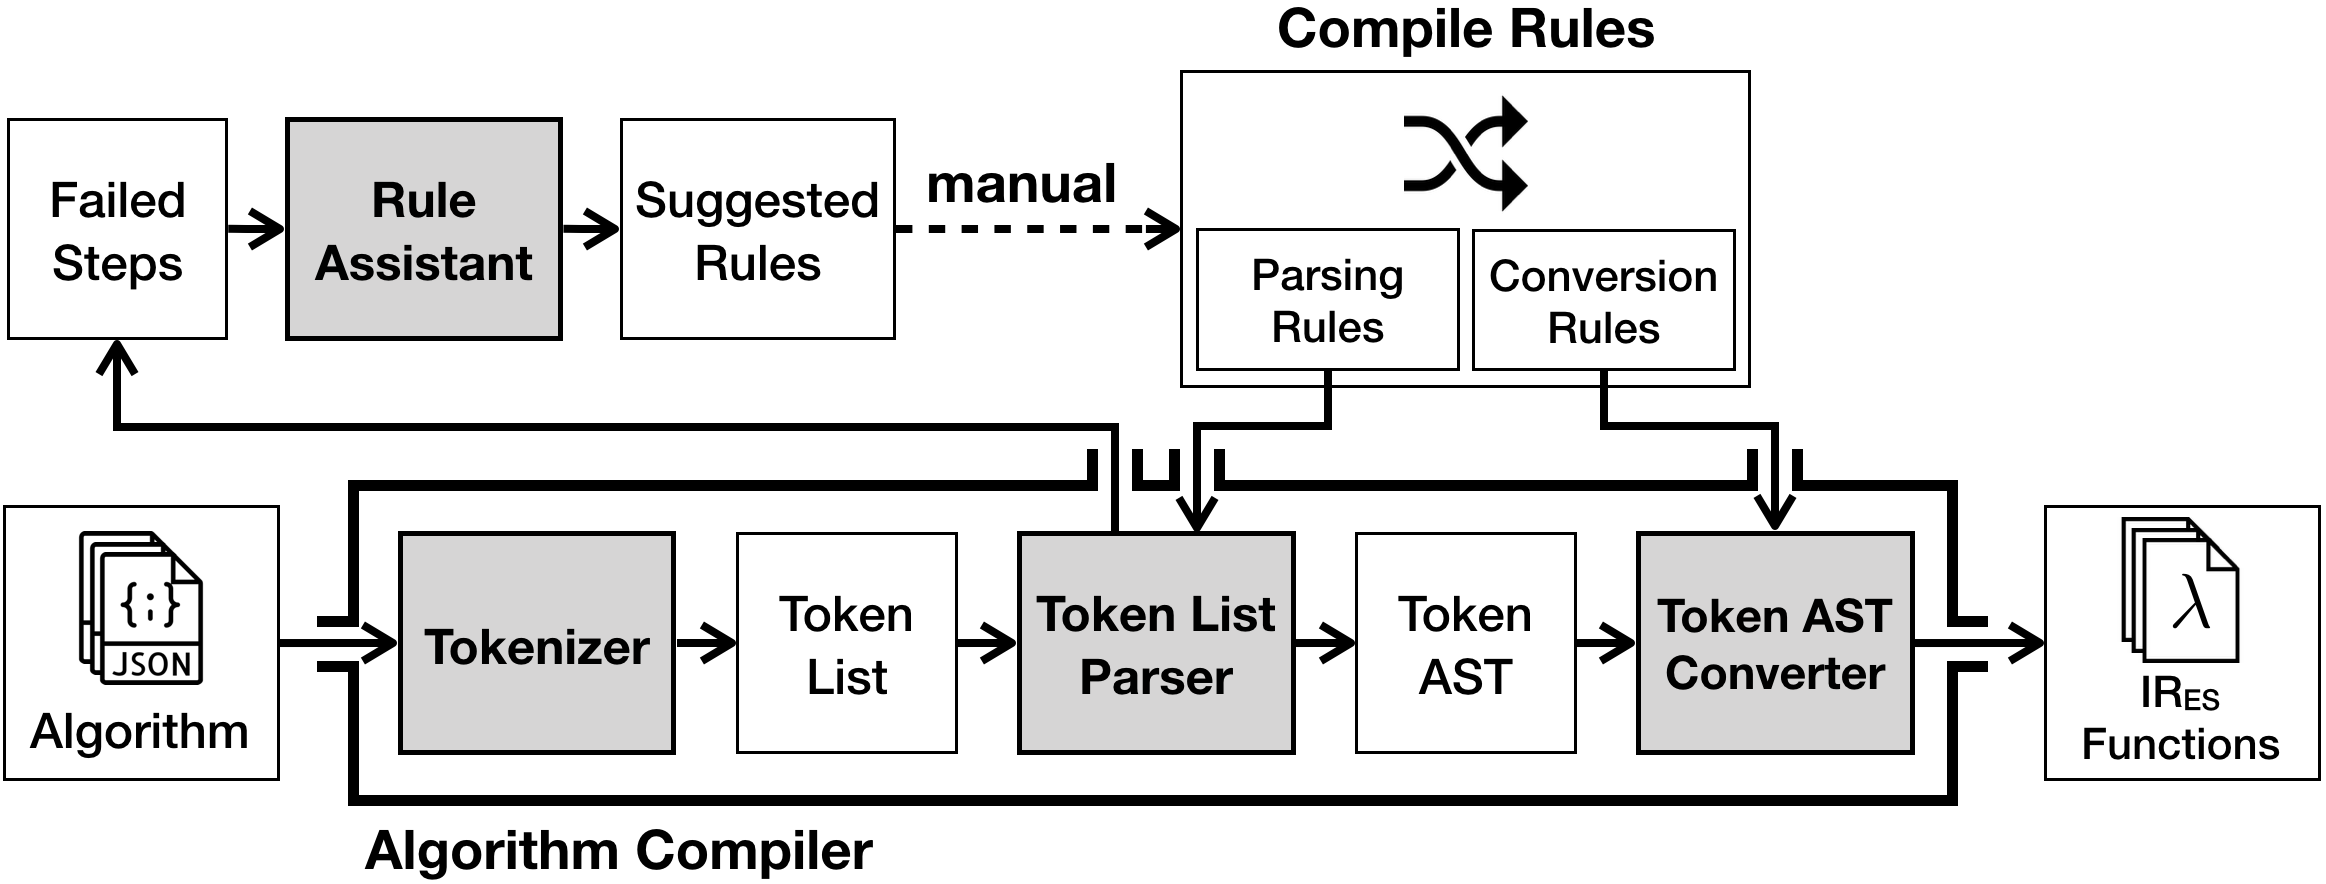
\includegraphics[width=0.5\textwidth]{img/algo_compiler.png}
  \caption{Overall structure of the algorithm compiler.}
  \label{fig:algo-compiler}
\end{figure}

In this section, we propose the \textit{algorithm compiler}
that compiles abstract algorithms into \( \ires \) functions
and its overall structure is described in Figure~\ref{fig:algo-compiler}.
Before compiling abstract algorithms,
the tokenizer first tokenizes each abstract algorithm into
a list of tagged tokens. Then, the token parser constructs
syntactic parse tree of the given token list.
Finally, the \( \ires \) function generator constructs the coressponding
\( \ires \) function from the given parse tree.
The parser and the generator is dependent on conversion rules
and we define the general conversion rules for abstract algorithms in
ECMAScript specifications. Like Coq, a proof assistant, we also provide
the \textit{rule generation assistant} to make easy write conversion rules.
It diagnoses root causes of failed parsing tokens
and suggests new conversion rules based on
statistical analysis of algorithm steps that failed to be parsed.

\subsection{Tokenizer}

Abstract algorithms in ECMAScript specifications are written in structured
natural languages in HTML files. An algorithm consists of ordered steps
and it might contain sub-steps as well. For example,
the \( \code{ToPrimitive} \) algorithm in Figure~\ref{fig:to-primitive-es}
has three steps and second step has seven sub-steps.
Moreover, the tokens of each step has its own HTML tag and each tag
has the following meaning:
\[
  \begin{array}{c|l}
    \text{HTML tags} & \text{meanings}\\\hline\hline
    \code{<var>} & \text{variables}\\\hline
    \code{<emu-grammar>} & \text{productions}\\\hline
    \code{<emu-nt>} & \text{non-terminal syntax}\\\hline
    \code{<code>} & \text{ECMAScript codes}\\\hline
    \code{<emu-const>} & \text{constant values}\\\hline
    \code{<emu-val>} & \text{values}\\\hline
    \code{<ol>} & \text{ordered sub-steps}\\\hline
    \code{<ul>} & \text{unordered sub-steps}\\\hline
    \code{<sup>} & \text{superscripts}\\\hline
    \text{otheriwse} & \text{simple texts}\\\hline
  \end{array}
\]
We try to keep the tag information for each token to generate more
precise conversion rules. For example, if and only if a token has a tag
\( \code{<var>} \), it is a parameter or a local variable.
Thus, it is possible to construct a conversion rule precisly discriminates
identifiers and other components.

The tokenizer first recognizes the overall structures of steps.
Then, it divides each step into sequence of tagged tokens.
If an HTML element has a explicit tag, it is converted into a single token
with the tag. Otherwise, it is splitted into multiple tokens and each token
should be a sequence of alphanumeric characters or a single
non-alphanumeric character. For example, in the \( \code{ToPrimitive} \)algorithm,
\( \textbf{\code{"default"}} \) is a single token with the tag \( \code{<code>} \)
and \( \code{@@toPrimitive} \) is splitted into three text tokens
\( \code{@} \), \( \code{@} \), and \( \code{toPrimitive} \).

For the linear structures, the tokenizer flatten the structured steps into
a single list. Some conversion rules should handle multiple steps such as
the conditional statements (if-then-else). Thus, we decide to break down
structured algorithms using three special tokens;
\( \tend \) denotes the end of a single step,
\( \tin \) and \( \tout \) the start and the end of nested steps, respectively.
For example, the \( \code{ToPrimitive} \) algorithm is tokenized as follows.
\[
  \begin{array}{l}
    \code{Assert} \cdots \tend\\
    \code{If} \cdots \tin \code{If} \cdots \tend
    \cdots \code{Return} \cdots \tend \tout \tend\\
    \code{Return} \cdots \tend\\
  \end{array}
\]

\subsection{Token Parser}

The token parser parses a given list of tokens into a syntactic parse tree.
It depends on the given \textit{conversion rules} that consists of
two parts parsing rules and mapping from parsing rules into corresponding
\( \ires \) components.
A parsing rule consists of basic token matchers and other parsing rules
including itself. For example, the following parsing rule is simplifed version for
sub-step \( i \) in the \( \code{ToPrimitive} \) algorithm.
\begin{lstlisting}[style=myScalastyle]
// statements
val Stmt = "Let" ~ varT ~ "be" ~ Expr ~ "." ^^ ...
// expressions
val Expr = (
  // identifiers
  varT ^^ ... |
  // return if abrupt
  "?" ~ Expr ^^ ... |
  // function calls
  textT ~ "(" ~ repsep(varT, ",") ~ ")" ^^ ... |
  // lists
  "<<" ~ repsep(Expr, ",") ~ ">>" ^^ ...
)
\end{lstlisting}

Each parsing rule is written in extended Scala parser combinators.
We modify the meaning of altenative composition operator ( \( | \) ) to collect
all longest matched results. If the parser detects that a step cannot be
parsed with the given parsing rules. It reports that a step is not possible
to be parsed under the given rules into the rule generation assistant.
Moreover, even though the parser could parse a step, it will be also reported
if it could be parsed in not a single but multiple ways.
Each string literal is a token matcher for tokens without any tags and checks
that the token has same string value with the sring literal.
The \( \code{varT} \) and \( \code{textT} \) is also token matchers
for token with the tag \( \code{<var>} \) and no tags.
The \( \code{Step} \) and \( \code{Expr} \) are user-defined parsing rules
defined with our extended parser combinators.
Morevoer, it supports all helpers functions defined in Scala parser combinators.
For example, the helper function \( \code{repsep(p, q)} \) generates a new
parsing rule that denotes zero or more repetitions of the parsing rule \( \code{p} \)
using another parsing rule \( \code{q} \) as separators.
Finally, the token parser with the above rules parses sub-step \( i \) in the
\( \code{ToPrimitive} \) into the following syntactic parse tree:
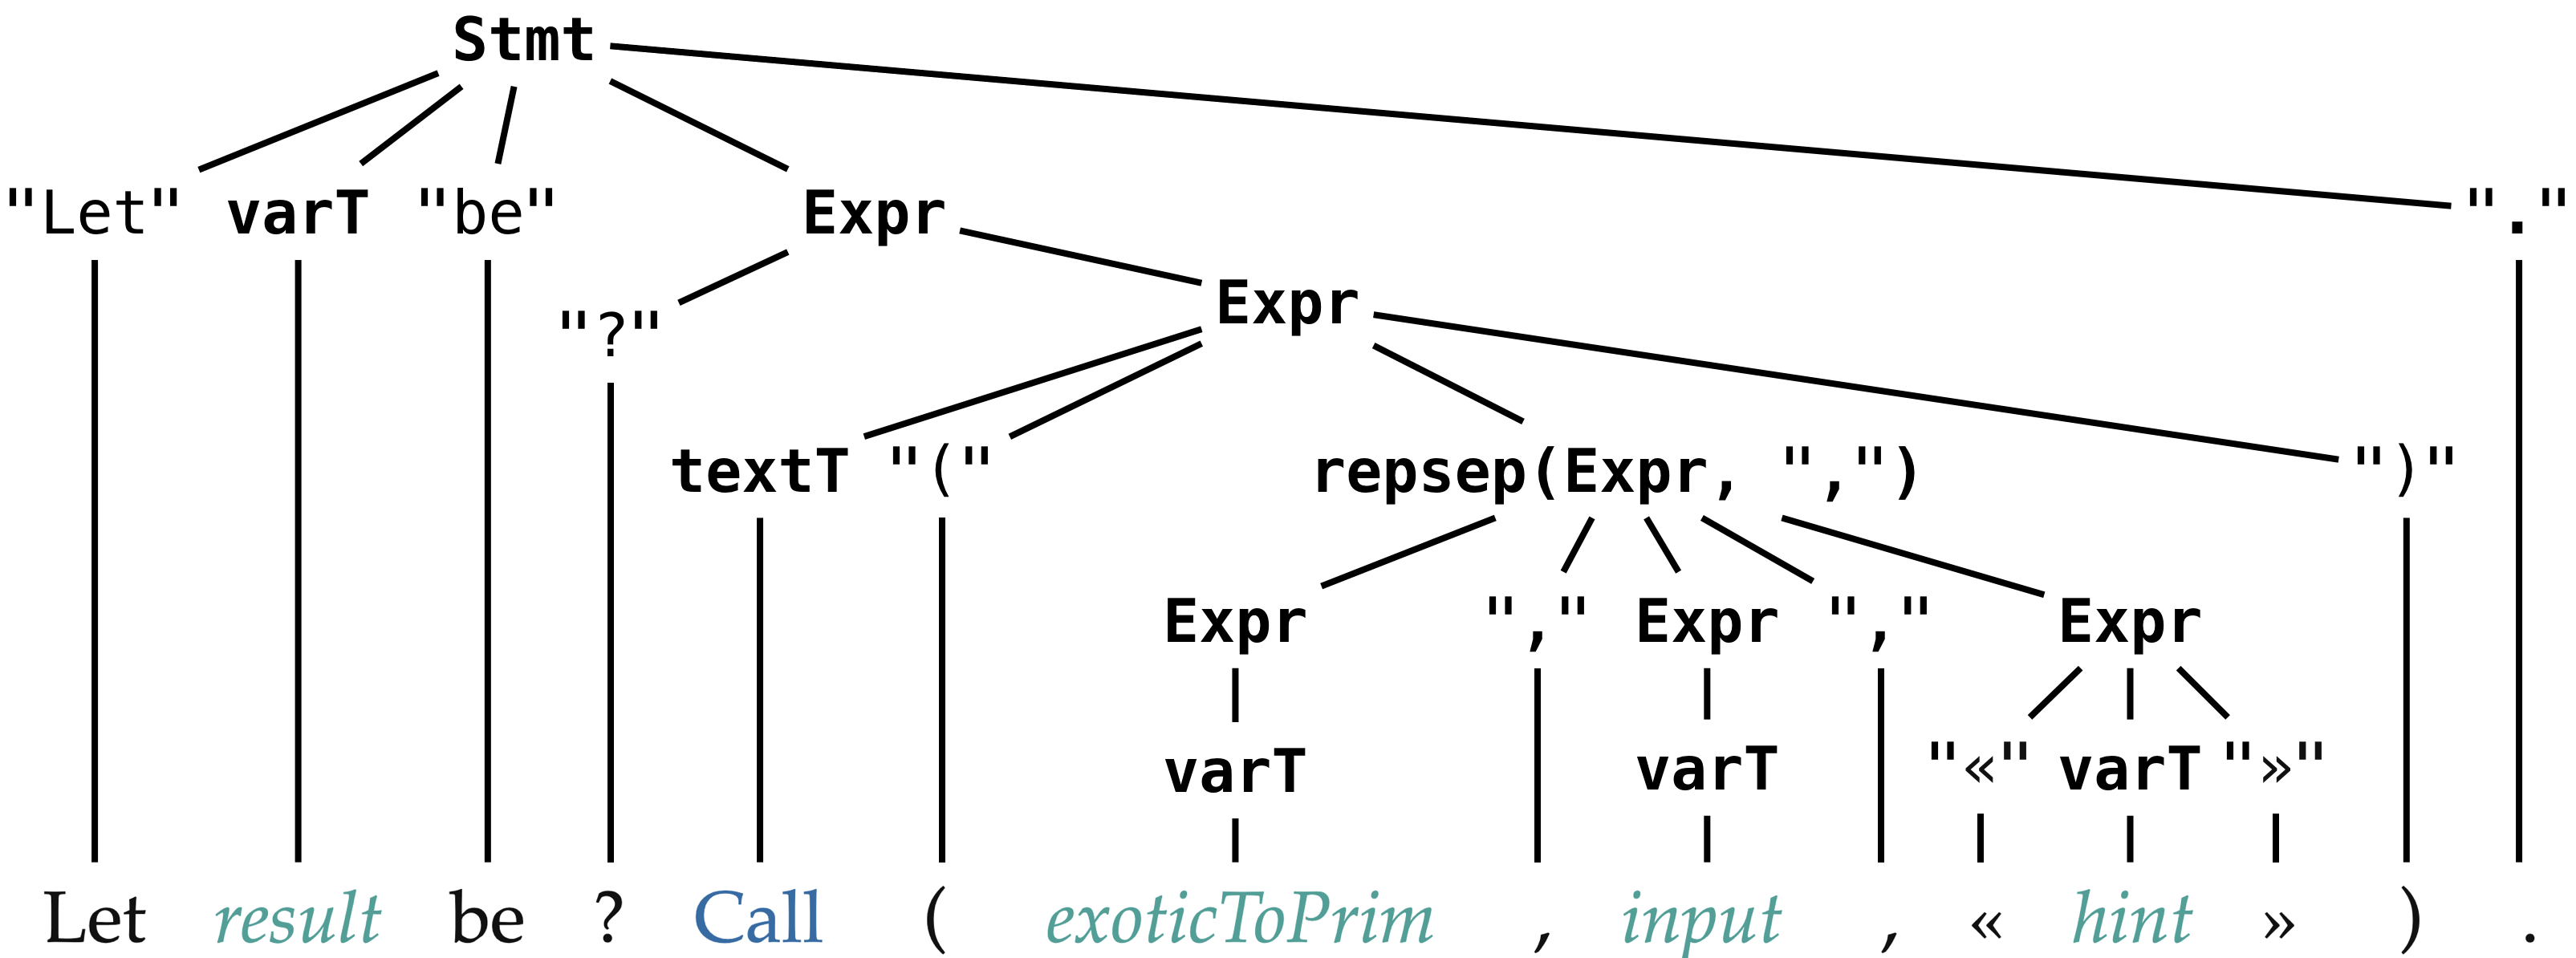
\includegraphics[width=0.5\textwidth]{img/parse_tree.png}

\subsection{\( \ires \) Function Generator}

We define \( \ires \) language to give semantics into syntactic parse tree of
abstract algorithm steps. It has the following language features:

\begin{itemize}
\item \textbf{Dynamic Typing} We decide to use dynamic typing for \( \ires \)
because each variables in abstract algorithms are not statically typed.
Thus, variables do not have its own static types while each value of \( \ires \)
has its dynamic type.

\item \textbf{Imparative Style} \( \ires \) represents algorithm steps
as statements. Each statement changes the current state
that consists of environments and a heap.

\item \textbf{Higher-order Functions with Restricted Scopes} \( \ires \) supports
lambda functions as values but it has only restricted scopes. In each function,
only global variables, parameter, and newly defined local variables are accessible.
It means that the function closure does not capture the the current environemnt.
We use such restricted scopes becuase it is enough to represent abstract algorithms.

\item \textbf{Primitive Values} \( \ires \) supports ECMAScript primitive values except
the symbols that is newly introduced after ECMAScript 6. Thus, only five ECMAScript primitives
are defined in \( \ires \); numbers, strings, booleans, undefined, and null.
Moreover, \( \ires \) also supports the unique \( \code{absent} \) value to represent
the absence of parameters. For example, the second parameter \( \code{PreferredType} \)
of \( \code{ToPrimitive} \) algorithm in Figure~\ref{fig:to-primitive-es} might be
not present in some function calls. Then, the parameter has the \( \code{absent} \) value
to represent its absence.

\item \textbf{Abstract Data Types} \( \ires \) only supports three abstract data types;
\( \code{Record} \) for mapping from some values into other value,
\( \code{List} \) for sequenital data types,
and \( \code{Singletone} \) for singleton data types.
They are stored in corresponding addresses in the heap structure.
For example, ECMAScript environment records are represented as \( \code{Record} \) data types
from String values for identifier names into addresses.
The addresses point to other \( \code{Record} \) data types that represent ECMAScript bindings.
We treat a ECMAScript constants such as \( \code{empty} \) and primitive symbols as singleton
data types in \( \ires \).
\end{itemize}

To generate the corresponding \( \ires \) function from syntactic parse tree,
we describe the mapping from each parsing rule into the corresponding \( \ires \) components.
For example, we describe the following mapping for the previous example parsing rules:
\begin{lstlisting}[style=myScalastyle]
// statements
val Stmt = ... ^^ { case _ ~ x ~ _ ~ y => ESLet(x, y) }
// expressions
val Expr = (
  // identifiers
  ... ^^ { x => x } |
  // return if abrupt
  ... ^^ { _ ~ e => ESReturnIfAbrupt(e) } |
  // function calls
  ... ^^ { case x ~ _ ~ y ~ _ => ESCall(x, y) } |
  // lists
  ... ^^ { case _ ~ x ~ _ => ESList(e) }
)
\end{lstlisting}
Finally, sub-step \( i \) in the \( \code{ToPrimitive} \) is converted
into the following instruction:
\begin{lstlisting}[style=ires]
let result = ? (Call exoticToPrim input (new [hint]))
\end{lstlisting}

\subsection{Rule Generation Assistant}

To make easy write conversion rules, we support \textit{rule generation assistant}.
It consists of several helper functions to show the specific statistics of
the not yet convertable abstract algorithm steps. It make easy not only construct
conversion reuls from the scratch but also update existing conversion rules
for updated specifications. We explain each helper function and how to utilize
it to construct conversion rules.

\subsubsection{Statement format suggestions}

\inred{TODO}

\subsubsection{Fault localizations based on \( \tstar \) tokens}

\inred{TODO}
